\documentclass[a4paper]{article} 
\usepackage{algorithm}
\usepackage{algpseudocode}

\addtolength{\hoffset}{-2.25cm}
\addtolength{\textwidth}{4.5cm}
\addtolength{\voffset}{-3.25cm}
\addtolength{\textheight}{5cm}
\setlength{\parskip}{0pt}
\setlength{\parindent}{0in}

%----------------------------------------------------------------------------------------
%	PACKAGES AND OTHER DOCUMENT CONFIGURATIONS
%----------------------------------------------------------------------------------------

\usepackage{blindtext} % Package to generate dummy text
\usepackage{charter} % Use the Charter font
\usepackage[utf8]{inputenc} % Use UTF-8 encoding
\usepackage{microtype} % Slightly tweak font spacing for aesthetics
\usepackage[english]{babel} % Language hyphenation and typographical rules
\usepackage{amsthm, amsmath, amssymb} % Mathematical typesetting
\usepackage{float} % Improved interface for floating objects
\usepackage[final, colorlinks = true, 
            linkcolor = black, 
            citecolor = black]{hyperref} % For hyperlinks in the PDF
\usepackage{graphicx, multicol} % Enhanced support for graphics
\usepackage{xcolor} % Driver-independent color extensions
\usepackage{marvosym, wasysym} % More symbols
\usepackage{rotating} % Rotation tools
\usepackage{censor} % Facilities for controlling restricted text
\usepackage{listings, style/lstlisting} % Environment for non-formatted code, !uses style file!
\usepackage{pseudocode} % Environment for specifying algorithms in a natural way
\usepackage{style/avm} % Environment for f-structures, !uses style file!
\usepackage{booktabs} % Enhances quality of tables
\usepackage{tikz-qtree} % Easy tree drawing tool
\tikzset{every tree node/.style={align=center,anchor=north},
         level distance=2cm} % Configuration for q-trees
\usepackage{style/btree} % Configuration for b-trees and b+-trees, !uses style file!
\usepackage[backend=biber,style=numeric,
            sorting=nyt]{biblatex} % Complete reimplementation of bibliographic facilities
\addbibresource{ecl.bib}
\usepackage{csquotes} % Context sensitive quotation facilities
\usepackage[yyyymmdd]{datetime} % Uses YEAR-MONTH-DAY format for dates
\renewcommand{\dateseparator}{-} % Sets dateseparator to '-'
\usepackage{fancyhdr} % Headers and footers
\pagestyle{fancy} % All pages have headers and footers
\fancyhead{}\renewcommand{\headrulewidth}{0pt} % Blank out the default header
\fancyfoot[L]{} % Custom footer text
\fancyfoot[C]{} % Custom footer text
\fancyfoot[R]{\thepage} % Custom footer text
\newcommand{\note}[1]{\marginpar{\scriptsize \textcolor{red}{#1}}} % Enables comments in red on margin

%----------------------------------------------------------------------------------------


\begin{document}

%-------------------------------
%	TITLE SECTION
%-------------------------------

\fancyhead[C]{}
\hrule \medskip % Upper rule
\begin{minipage}{0.295\textwidth} 
\raggedright
\footnotesize
Giacomo Mariani \hfill\\   
545519 \hfill\\
g.mariani16@studenti.unipi.it
\end{minipage}
\begin{minipage}{0.4\textwidth} 
\centering 
\large 
SPM final project -- A. A. 2020/21\\ 
\normalsize 
Free Choice -- PRUDEnce \\ 
\end{minipage}
\begin{minipage}{0.295\textwidth} 
\raggedleft
\today\hfill\\
\end{minipage}
\medskip\hrule 
\bigskip

%-------------------------------
%	CONTENTS
%-------------------------------

\section{Problem presentation}
The PRUDEnce (Privacy Risk vs Utility in data sharing Environment) algorithm can be used to compute the empirical privacy risk of a user when his/her contents are inserted into a public dataset, even when the user informations are pseudonymized using a unique identifier.
The algorithm takes in input a dataset $D$ composed by a sequence of records in the following form:
$$
    \left < u; p_1, p_2 \dots p_m \right >
$$

$u$ is the unique identifier that represents a user, such as a numeric key or a username string, and $p_1 \dots p_m$ are the \textit{features}, arbitrarily complex data structures for which we can define a notion of \textit{matching}. In the implementation I will focus on simple numerical values coming from the natural language processing of the Enron dataset, where every feature is associated to a special lexical characteristic and we indicate the matching of two features with the following function:
$$
    m(p[j], q[j]) = \begin{cases}
        1, & p[j] \in [q[j] - \epsilon \cdot q[j], q[j] + \epsilon \cdot q[j]]\\
        0, & \text{otherwise}
    \end{cases}
$$

The \textit{reidentification attack} presented in the paper proceeds as follows:
\begin{enumerate}
    \item The attacker has a \textit{background knowledge} composed of a subset $t = \{ q_{j_1}, q_{j_2} \dots q_{j_h} \}$ of $h$ features referred to a user, representing the fact that the attacker knows that the addressed user has certain characteristics inserted into the dataset.
    \item The attacker scans the whole dataset looking for users where the subset of the feature values matches with the one in the background knowledge, meaning that the matching user may be the one that has to be reidentified. The set of matching users is defined as:
    $$
        R_t = \{ v\ |\ \left < v; q_1 \dots q_m \right > \in D \land m(p[j_1], q[j_1]) = 1 \land \dots \land m(p[j_h], q[j_h]) = 1 \}
    $$
    \item If $R_t = \{ u \}$, the unknown user is surely reidentified as $u$, and the attack succeeded. If $R_t = \{ u_1 \dots u_m \}$ we have more choices, so the background knowledge is not sufficient.
\end{enumerate}

Given a background knowledge $t$ we can hence define the \textit{probability of reidentification} of a user $u$ as:
$$
    PR(u|t) = \frac{1}{|R_t|}
$$

\begin{algorithm}
    \begin{algorithmic}
        \Function{ProbReidentification}{$\left < u; p \right >, D, \left \{ j_1 \dots j_h \right \}$}
            \State $matches \gets 0$
            \For{$\left < v; q \right > \in D$}
                \State $m \gets 1$
                \For{$j \in \left \{ j_1 \dots j_h \right \}$}
                    \If{$m(p[j], q[j]) = 0$}
                        \State $m \gets 0$
                        \State \textbf{break}
                    \EndIf
                \EndFor
                \State $matches \gets matches + m$
            \EndFor
            \State \textbf{return} $1 / matches$
        \EndFunction
    \end{algorithmic}
    \caption{Probability of reidentification of a user in the dataset w.r.t. a background knowledge}
    \label{algo:prob-reidentification}
\end{algorithm}

The pseudocode to compute the probability of reidentification is detailed in the Algorithm \ref{algo:prob-reidentification}. Note that in the implementation, in order to avoid handling floating point numbers, we returned the number of matches instead of the probability.

We denote with $t_M$ the time spent to match two features, and since to compute a single probability of reidentification we have to match $h$ features for $n$ records we have that the time spent to compute \textsc{ProbReidentification} is $T_P \le n \cdot h \cdot t_M$. Note that this is an upper bound, and depending on the data, early stoppings might be very common.

We denote the set of all the possible background knowledges extractible from $D$ as:
$$
    BK_h = \{t = \{p_{j_1} \dots p_{j_h}\} \in D\ |\ \{j_1 \dots j_h\} \text{ is a combination of } h \text{ elements of } \{1 \dots m\}\}
$$

The \textit{risk of reidentification} of a user is hence defined as the maximum probability of reidentification on $D$ for all the possible background knowledge instances:
$$
    Risk_D(u, h) = \max\limits_{t \in BK_h} PR(u|t) = \max\limits_{t \in BK_h} \frac{1}{|R_t|}
$$
\begin{algorithm}
    \begin{algorithmic}
        \Function{AssessRisk}{$\left < u; p \right >, D, h$}
            \State $risk \gets -\infty$
            \For{$\left \{ j_1 \dots j_h \right \} \text{ combination of } h \text{ indices of }\left \{ 1 \dots m \right \}$}
                \State $prob \gets$ \textsc{ProbReidentification}($\left < u; p \right >, D, \left \{ j_1 \dots j_h \right \}$)
                \If{$prob = 1$}
                    \State \textbf{return} 1
                \EndIf
                \State $risk \gets \max \left \{ risk, prob \right \}$
            \EndFor
            \State \textbf{return} $risk$
        \EndFunction
    \end{algorithmic}
    \caption{Risk of reidentification for a user in the dataset w.r.t. a background knowledge size}
    \label{algo:risk-reidentification}
\end{algorithm}

In Algorithm \ref{algo:risk-reidentification} you can find the pseudocode to compute the risk of reidentification for a user in the dataset considering a certain background knowledge size.

Since the possible combinations of $h$ indices are $\binom{m}{h}$, to compute \textsc{AssessRisk} we need $T_A \le n \cdot \binom{m}{h} \cdot h \cdot t_M$. Note that this is again an upper-bound.

\begin{algorithm}
    \begin{algorithmic}
        \Function{AssessRiskDataset}{$D, h$}
            \For{$\left < u; p \right > \in D$}
                \State $r \gets$ \textsc{AssessRisk}($\left < u; p \right >, D, h$)
                \State \textbf{output} $\left < u, r \right >$
            \EndFor
        \EndFunction
    \end{algorithmic}
    \caption{Risk assessment for a whole dataset}
    \label{algo:risk-dataset}
\end{algorithm}

For this project, we choose to fix the background knowledge size and to compute the risk for the whole dataset, as detailed in Algorithm \ref{algo:risk-dataset}. In this way we obtain that to compute \textsc{AssessRiskDataset} we need a time, expressed in terms of \textit{latency}:
$$
	T_{seq} = L \le n^2 \cdot \binom{m}{h} \cdot h \cdot t_M
$$

\section{Parallel implementation}

The first thing we can observe is that, to start computing the first risk, the whole dataset has to be loaded in main memory, so it's not possible to parallelize the reading phase using a pipeline. For simplicity, we decided to keep in main memory also the output vector, and then to serialize it altogether.

A parallel implementation of the algorithm can exploit the fact that \textsc{AssessRiskDataset} can be implemented as a \texttt{map} of \textsc{AssessRisk} on each element of $D$, or similarily as a special case of \texttt{stencil} that involves the whole dataset. This can be parallelized by a farm of workers computing the function, possibily coordinated by an emitter. Each worker is assigned to a specific chunk of users, accesses $D$ read-only, and similarily writes the risk in an array following the \textit{owner-only-writes} rule, so there is no need for synchronization between the concurrent entities. In total, with a parallelism degree of $nw$, each worker computes $\frac{n}{nw}$ values. A graphical representation of this schema is depicted in Figure \ref{fig:schema}.

\begin{figure}
    \centering
    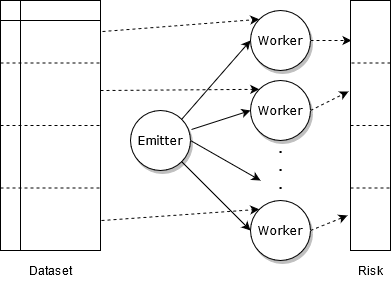
\includegraphics[scale=0.7]{img/Schema.png}
    \caption{Logical schema of the parallel application}
    \label{fig:schema}
\end{figure}

\subsection{Static scheduling}

In the simplest version, we compute the function in an \textit{embarassingly parallel} way. Each worker is assigned to a chunk of the dataset, and for each record in the chunk computes risk and writes it into the output array. The emitter's only task is to split the dataset into chunks and spawn the workers taking a time $t_{split}$ per worker, and then join them at the end of the computation with a time $t_{merge}$ per worker. The latency in this case is:
$$
    T_{par}^S(nw) \le nw \cdot \left ( t_{split} + t_{merge} \right ) + \frac{n^2}{nw} \cdot \binom{m}{h} \cdot h \cdot t_M
$$

We can then measure how the performances increase when we add more workers:
$$
    speedup^S(nw) = \frac{T_{seq}}{T_{par}^S(nw)} \le \frac{n^2 \cdot \binom{m}{h} \cdot h \cdot t_M}{nw \cdot \left ( t_{split} + t_{merge} \right ) + \frac{n^2}{nw} \cdot \binom{m}{h} \cdot h \cdot t_M}
$$
Being a function of this form, the speedup reaches a peak value, then the overhead factor becomes dominant and the quantity decreases down to zero:
$$
    \lim \limits_{nw \to \infty} speedup^S(nw) = \lim \limits_{nw \to \infty} \frac{n^2 \cdot \binom{m}{h} \cdot h \cdot t_M}{nw \cdot \left ( t_{split} + t_{merge} \right ) + \frac{n^2}{nw} \cdot \binom{m}{h} \cdot h \cdot t_M} = 0
$$

We can also measure how this parallel implementation is able to exploit the available resources, defining the efficiency:
$$
    \epsilon^S(nw) = \frac{T_{id}(nw)}{T_{par}^S(nw)} = \frac{speedup^S(nw)}{nw} \le \frac{n^2 \cdot \binom{m}{h} \cdot h \cdot t_M}{nw^2 \cdot \left ( t_{split} + t_{merge} \right ) + n^2 \cdot \binom{m}{h} \cdot h \cdot t_M}
$$
This quantity rapidly decreases down to zero when the parallelism degree increases:
$$
    \lim \limits_{nw \to \infty} \epsilon^S(nw) = \lim \limits_{nw \to \infty} \frac{n^2 \cdot \binom{m}{h} \cdot h \cdot t_M}{nw^2 \cdot \left ( t_{split} + t_{merge} \right ) + n^2 \cdot \binom{m}{h} \cdot h \cdot t_M} = 0
$$

Finally, we can measure how the implementation scales when the parallelism degree increases:
$$
    scalability^S(nw) = \frac{T_{par}^S(1)}{T_{par}^S(nw)} \le \frac{t_{split} + t_{merge} + n^2 \cdot \binom{m}{h} \cdot h \cdot t_M}{nw \left (t_{split} + t_{merge} \right ) + \frac{n^2}{nw} \cdot \binom{m}{h} \cdot h \cdot t_M}
$$
This function behaves like speedup, reaching a maximum value and then decreasing:
$$
    \lim \limits_{nw \to \infty} scalability^S(nw) = \frac{t_{split} + t_{merge} + n^2 \cdot \binom{m}{h} \cdot h \cdot t_M}{nw \left (t_{split} + t_{merge} \right ) + \frac{n^2}{nw} \cdot \binom{m}{h} \cdot h \cdot t_M} = 0
$$

Summing up, this kind of implementation can be convenient up to a certain parallelism degree, but cannot indefinitely scale due to the increasing overhead factor.

\subsection{Dynamic scheduling}

In the dataset $D$ might exist regions in which early stoppings are more frequent than in others, so it might be useful to introduce a dynamic scheduling of the chunks among the threads. This version introduces a feedback queue that the workers use to notify the emitter that they finished their assigned chunk and need a new one. The emitter satisfies these requests one after the other, until there is no more chunks to assign. Then for every new request it sends an End Of Stream (\texttt{EOS}) symbol, signaling the conclusion. In this case, the emitter has to be active all the time, employing a time $t_E$ for each worker. The parallel time becomes:
$$
    T_{par}^D(nw) \le \max \left \{ nw \cdot t_E, \frac{n^2}{nw} \cdot \binom{m}{h} \cdot h \cdot t_M \right \}
$$

Hence the speedup is bounded by the ratio between the sequential time and the emitter time:
$$
    speedup^D(nw) \le \frac{n^2 \cdot \binom{m}{h} \cdot h \cdot t_M}{\max \left \{ nw \cdot t_E, \frac{n^2}{nw} \cdot \binom{m}{h} \cdot h \cdot t_M \right \}} \implies \lim \limits_{nw \to \infty} speedup^D(nw) = 0
$$

Efficiency is heavily influenced by the $nw$ factor at the denominator:
$$
    \epsilon^D(nw) = \frac{speedup^D(nw)}{nw} \le \frac{n^2 \cdot \binom{m}{h} \cdot h \cdot t_M}{nw \cdot \max \left \{ nw \cdot t_E, \frac{n^2}{nw} \cdot \binom{m}{h} \cdot t_M \right \}} \implies \lim \limits_{nw \to \infty} \epsilon^D(nw) = 0
$$

For the scalability we have the same behaviour as in speedup, regulated by the $nw$ multiplicative factor of $t_E$:
$$
    scalability^D(nw) = \frac{T_{par}(1)}{T_{par}(nw)} \le \frac{\max \left \{ t_E, n^2 \cdot \binom{m}{h} \cdot h \cdot t_M \right \}}{\max \left \{ nw \cdot t_E, \frac{n^2}{nw} \cdot \binom{m}{h} \cdot h \cdot t_M \right \}} \implies \lim \limits_{nw \to \infty} scalability^D(nw) = 0
$$
Asymptotically speaking, there are no theoretical guarantees that a dynamic scheduling increases the performances of this application.

\section{Implementation details}

The business logic implementing the privacy risk assessment is included in the \texttt{lib/prudence} folder, with the \texttt{Record} class that provides all the methods needed to compute matching.

Four executables were provided for this project, two using the standard C++ Threads abstractions and two using FastFlow. For each one of the two versions, one uses a static load balancing strategy and the other uses a dynamic one, where each chunk is of size $\frac{n}{2 \cdot nw}$ (used for consistency between the C++ Threads and FastFlow versions).

All the four implementations take the following command line arguments:
\begin{verbatim}
    ./prudence_{version}_{scheduling} nw h input_filename output_filename [eps=0.3] [id_index=0]
\end{verbatim}
\begin{itemize}
    \item \texttt{nw}: Parallelism degree of the implementation. If the provided value is 0, the applications falls back to the sequential version.
    \item \texttt{h}: Size of the background knowledge.
    \item \texttt{input\_filename}: Filename of the input CSV file parsed as dataset.
    \item \texttt{output\_filename}: Filename of the CSV file in which the tuples $\left < u_i, r_i \right >$ are saved.
    \item \texttt{eps} (optional, defaults to 0.3): Epsilon used to compute the matching.
    \item \texttt{id\_index} (optional, defaults to 0): Index, starting from 0, that identifies the column that has to be stored as user ID and not as a feature.
\end{itemize}

The applications share the same structure: they read the input file, store it in an array of \texttt{Record} object, compute the risk and then write the tuples $\left < u_i, r_i \right >$ in the output CSV file.

\subsection{C++ Threads}

The versions using C++ standard thread abstractions are contained in \texttt{prudence\_threads\_static.cpp} and \texttt{prudence\_threads\_dynamic.cpp}. Both chronometrate the latency using a custom \texttt{UTimer} class contained in \texttt{lib/utimer.hpp}.

The static scheduling version forks $nw$ threads associated to a static chunk of the dataset. Each worker thread computes the risk for the chunk, mantaining a reference to the whole input vector (dataset) $D$, and writes the result in the output vector at the corresponding indices. In this context, the emitter's task is executed by the main thread, that performs the fork and join operations. This executable can be generated using the Makefile with \texttt{make prudence\_threads\_static}.

In the dynamic scheduling version, emitter and workers communicate via a thread safe queue implemented in \texttt{lib/safe\_queue.hpp}. The emitter sends the start and end indices of the assigned chunk to each worker using their own queue. The worker computes the risk for the received chunk and writes it, then inserts its own ID in a \textit{feedback} queue, signaling to the emitter that it needs another chunk to compute. The emitter pops the feedback queue and sends the new chunks as long as they arrive. If there are no more chunks to dispatch, the emitter sends a special End of Stream symbol. For this implementation the \texttt{std::optional} wrapper was exploited, so the \texttt{EOS} is represented by the special ``empty variable'' \texttt{\{\}}. To compile this executable we can issue the command \texttt{make prudence\_threads\_dynamic}.

\subsection{FastFlow}

The FastFlow implementation exploited the \texttt{ParallelFor} abstraction, implemented itself with a farm and an emitter. They use the \texttt{ffTime} function provided by the library to measure latency. The static scheduling version does not pass any argument as \texttt{chunk\_size} to the \texttt{parallel\_for} function, while the dynamic scheduling passes the value $\frac{n}{2 \cdot nw}$. These two versions can be compiled using the Makefile instructions \texttt{make prudence\_fastflow\_static} and \texttt{make prudence\_fastflow\_dynamic}.

\subsection{Benchmarking}

To evaluate the performances of the four versions, a Bash script is present in \texttt{benchmark.sh}. The script takes as input four command line parameters:
\begin{verbatim}
    ./benchmark.sh nw_max h input_filename output_filename
\end{verbatim}
\begin{itemize}
    \item \texttt{nw\_max}: Maximum parallelism degree to test for the four executables.
    \item \texttt{h}: Background knowledge size.
    \item \texttt{input\_filename}: Filename of the input CSV file.
    \item \texttt{output\_filename}: Filename of the CSV where to put the output.
\end{itemize}
The script produces an output in the form of a CSV file, and performs the following steps: at first it executes the sequential script and saves the sequential latecy, then it doubles the parallelism degree from 1 to \texttt{nw\_max}, tests the four executables, saves the times and compares it with an ideal time, obtained dividing the sequential time by the number of workers.

To plot completion latency, speedup, efficiency and scalability, a Python script exploiting \texttt{Pandas} and \texttt{matplotlib} was provided in \texttt{plots.py}.

\section{Test results}

The tests were executed by taking the Enron dataset, a classical set of e-mails, well-studied by the natural language processing community. The text documents were analyzed using LIWC, a state-of-the art software for statistical NLP, that extracted 31 features corresponding to the (absolute or relative) frequency of certain categories of words and lexical constructs. Then the records were grouped by author and the vectors of features were reduced to their point-wise average. In order to reduce the computational time to something easy testable, for the benchmark we took only the first 1500 rows (1499 records plus the column names row, that gets skipped) and limited the background knowledge size $h$ to 2. In order to perform this tests, it's possible to use the associate Makefile instruction: \texttt{make benchmark}.

The tests were performed on two different machines:
\begin{itemize}
    \item Lenovo ThinkPad E595, AMD Ryzen 7 3700U processor, clock speed 2.30 GHz. 4 cores hyperthreaded, 8 processing elements in total.
    \item Server with Xeon Phi processor, clock speed 1015.726 MHz. 64 cores per socket, 4 threads per core, 256 processing elements in total.
\end{itemize}

The latency of all the provided implementations, measured in milliseconds, can be found in Table \ref{table:latency}.

\begin{table}
    \centering
    \scalebox{0.8}{
        \begin{tabular}{|l|l|cc|cc|l|}
        \hline
            Host & $nw$ & C++ Threads (Static) & C++ Threads (Dynamic) & FastFlow (Static) & FastFlow (Dynamic) & Ideal \\ \hline
            ThinkPad & Sequential &  &  &  &  & 68893.5 \\ \hline
             & 1 & 68152.4 & 67745.6 & 67614.3 & 70679.5 & 68893.5 \\
             & 2 & 42633.7 & 42305.5 & 48891.5 & 61767.8 & 34446.75 \\
             & 4 & 28745.7 & 27454.6 & 27418 & 28758.2 & 17223.375 \\
             & 8 & 18642.2 & 18755 & 18711.9 & 19963.4 & 8611.6875 \\ \hline
            XeonPhi & Sequential &  &  &  &  & 362284 \\ \hline
             & 1 & 399923 & 400426 & 398693 & 399718 & 362284 \\
             & 2 & 212340 & 214450 & 227132 & 214217 & 181142 \\
             & 4 & 110491 & 110895 & 108732 & 109187 & 90571 \\
             & 8 & 57675 & 58139.1 & 57279.4 & 57128.6 & 45285.5 \\
             & 16 & 30965 & 31606.2 & 29482.3 & 30553.4 & 22642.75 \\
             & 32 & 21420.1 & 18467 & 15613 & 16422.6 & 11321.375 \\
             & 64 & 14670.1 & 9839.27 & 8515.54 & 11093.2 & 5660.6875 \\
             & 128 & 28740.1 & 6552.25 & 6392.34 & 7140.21 & 2830.34375 \\
             & 256 & 62038.6 & 5443.97 & 5819.37 & 5827.77 & 1415.171875 \\ \hline
        \end{tabular}
    }
    \caption{Latency of the various versions}
    \label{table:latency}
\end{table}

In order to have a more clear idea of the performances, we provided a series of plots. Since it has a larger number of points, only the test results on the Xeon Phi were plotted in this report.
 
\begin{figure}
    \centering
    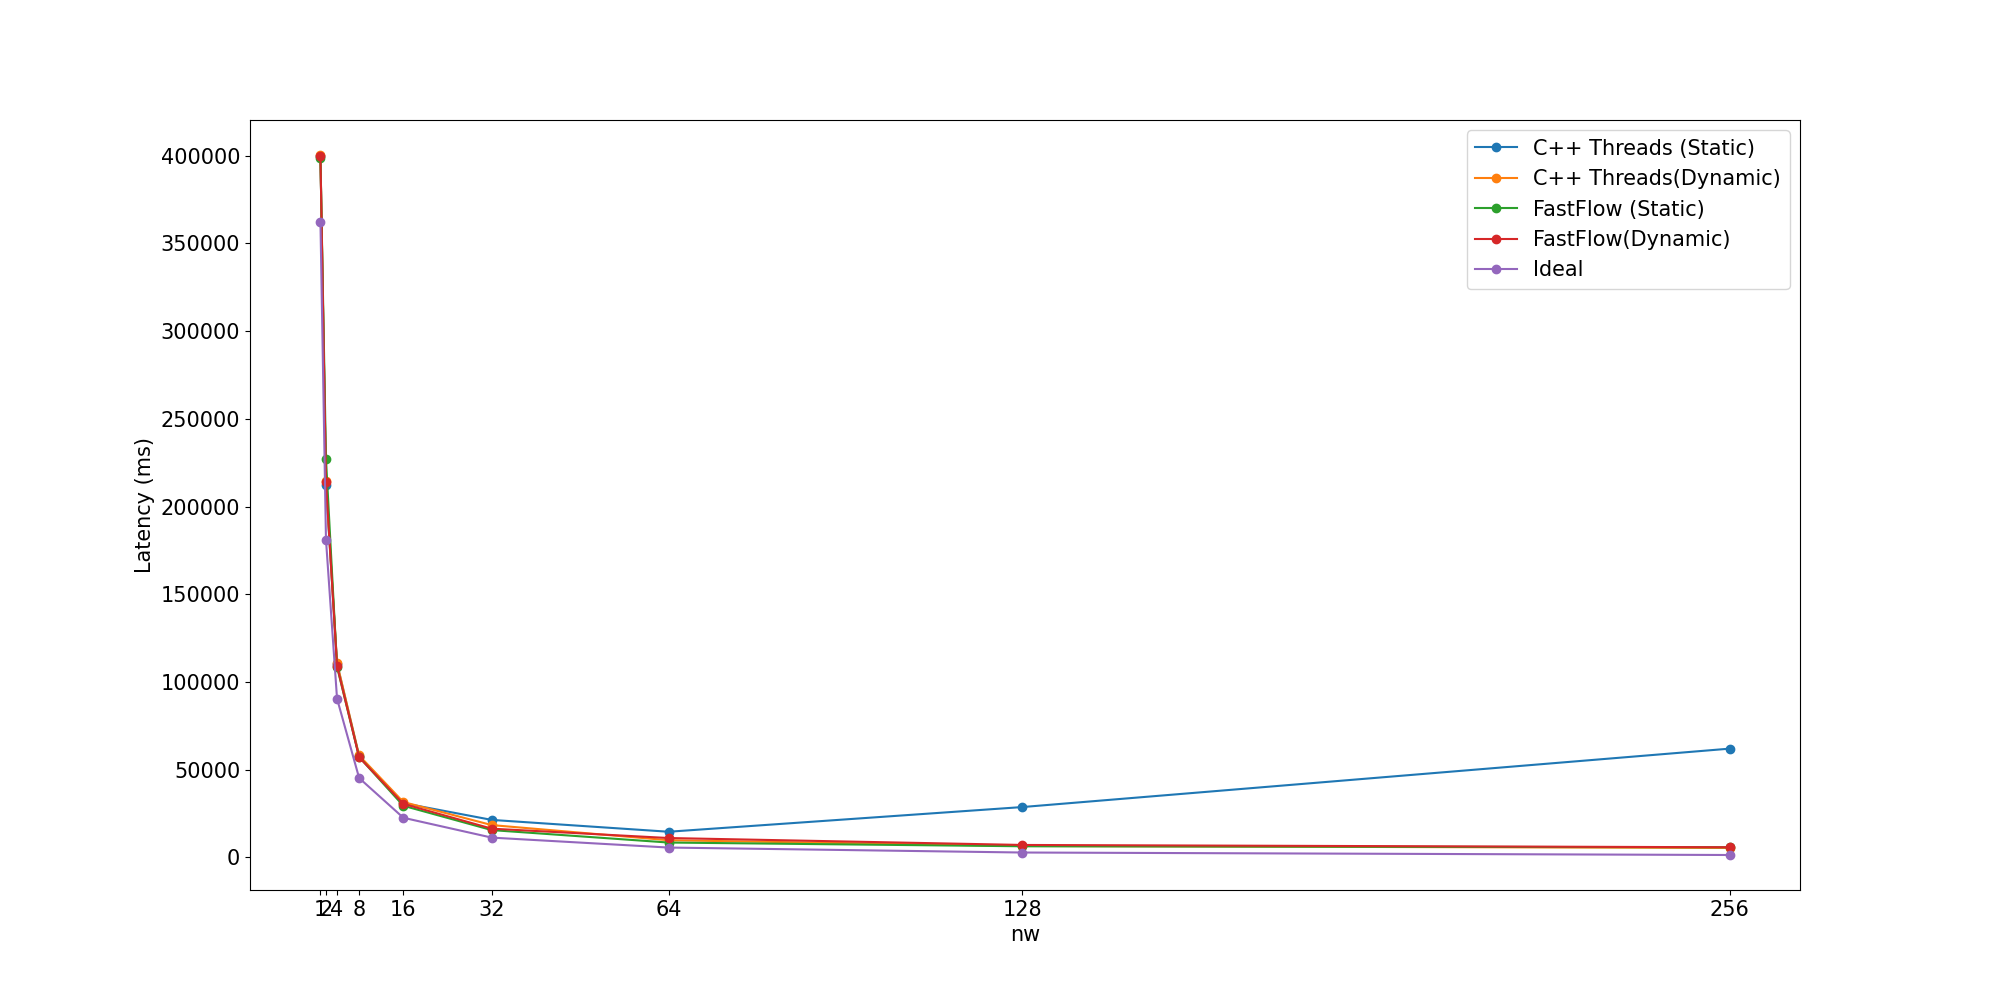
\includegraphics[width=\textwidth]{plots/latency.png}
    \caption{Latency on the Xeon Phi}
    \label{fig:latency}
\end{figure}

In Table \ref{table:latency} we can observe how the four versions decrease in latency more or less in the same way (near the ideal one), up to the point representing 64 worker threads. Increasing further the parallelism degree, all the implementations get similar latencies, except for the C++ Threads one using static scheduling, that rapidly degrades in performances. This can come from the fact that this version does not have any strategy to pin one thread to a specific core, so when the number of workers exceeds the physical amount of cores, a whole class of overhead operations are performed to enable context switches. Following this reasoning, we can hypotize that the dynamic scheduling version of the same implementation does not present this problem due to the fact that context switch is regulated mostly by the condition variables on the queue and not by a round-robin interleaving of threads that have to resume their job when respawned.

In general, we cannot extract the best performer watching this plot, but we can observe how \textit{by now} there is no clear winner between static and dynamic scheduling with these resources. Except from the already discussed outlier, the two strategies show very similar results.

\begin{figure}
    \centering
    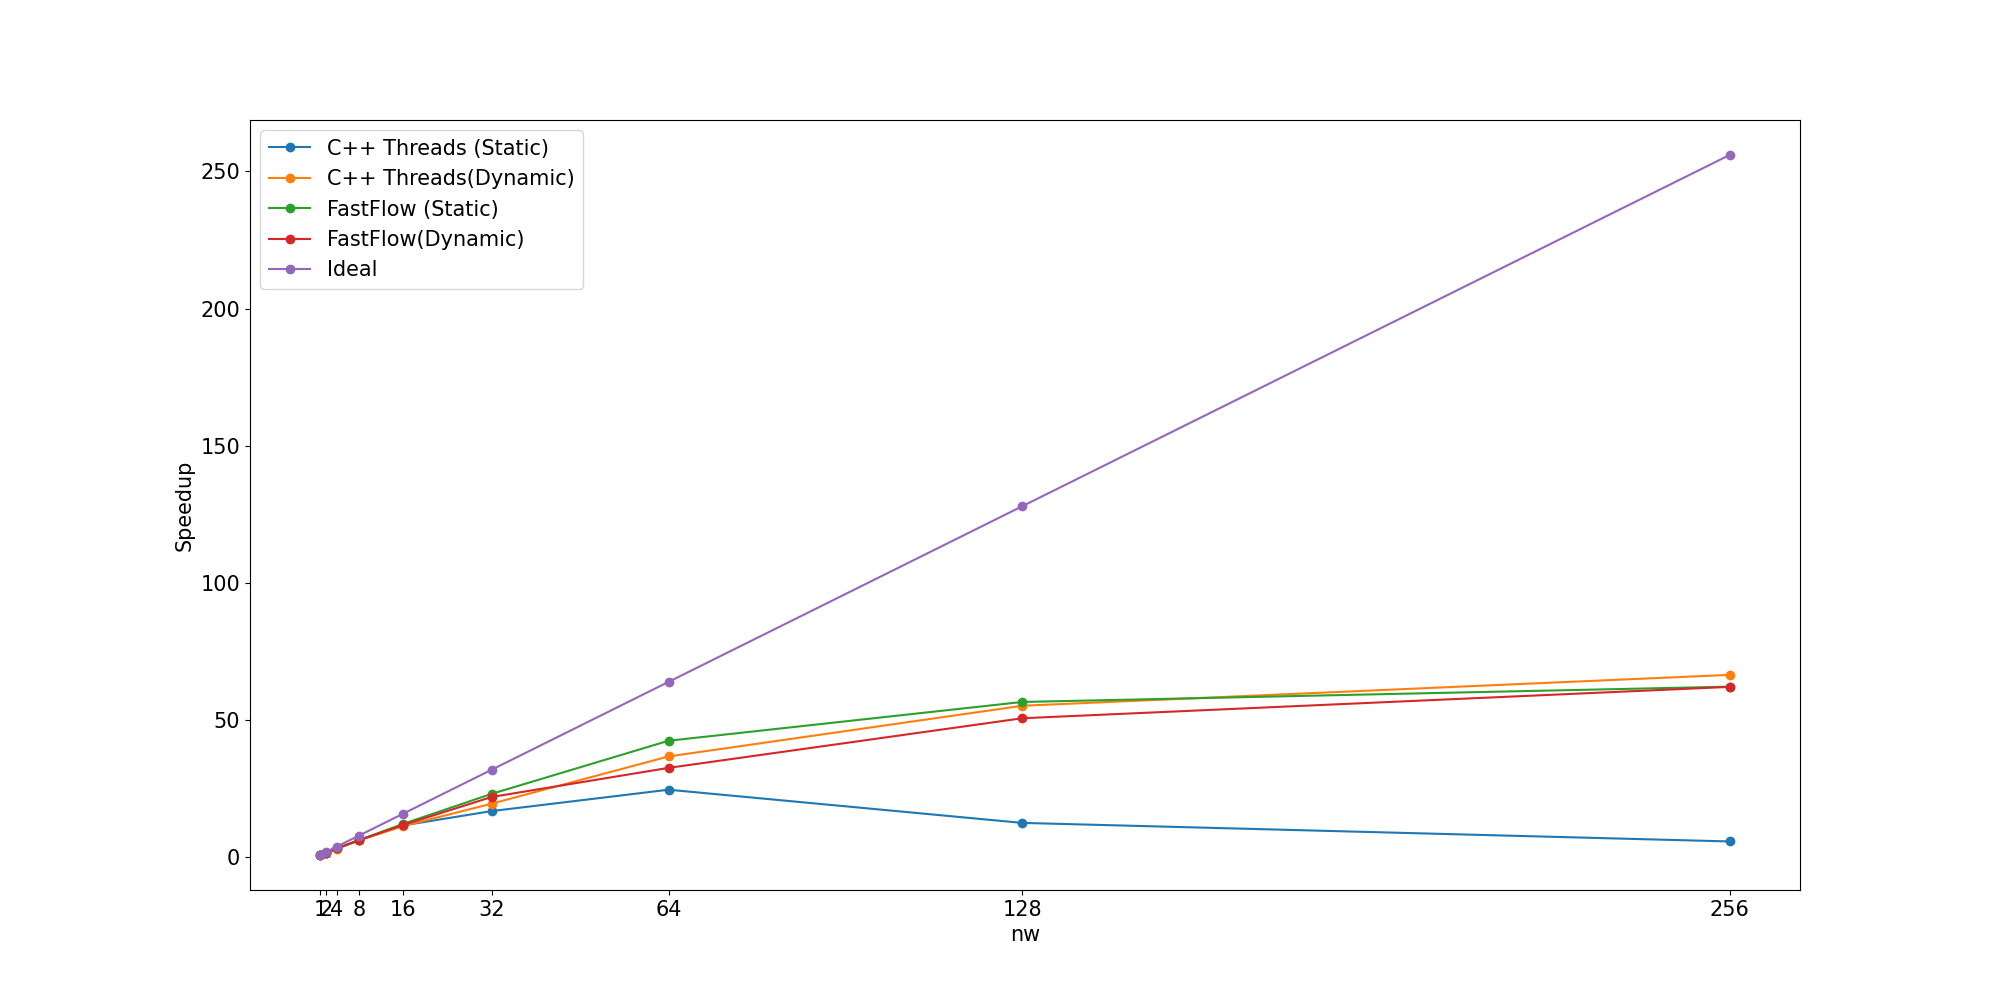
\includegraphics[width=\textwidth]{plots/speedup.png}
    \caption{Speedup on the Xeon Phi}
    \label{fig:speedup}
\end{figure}

Figure \ref{fig:speedup} shows how the FastFlow implementation with static strategy has the best speedup, but how this metric is heavily influenced by the overhead induced by the parallel implementation. In this case we can say that static scheduling is the best option for this setting, since the two dynamic versions mantain their curve clearly under the best performing one.

Speaking about the static scheduling, since the speedup keeps growing or stays the same for the two implementations, we have not yet reached the breakpoint beyond wich is no longer convenient to increase the parallelism degree.

\begin{figure}
    \centering
    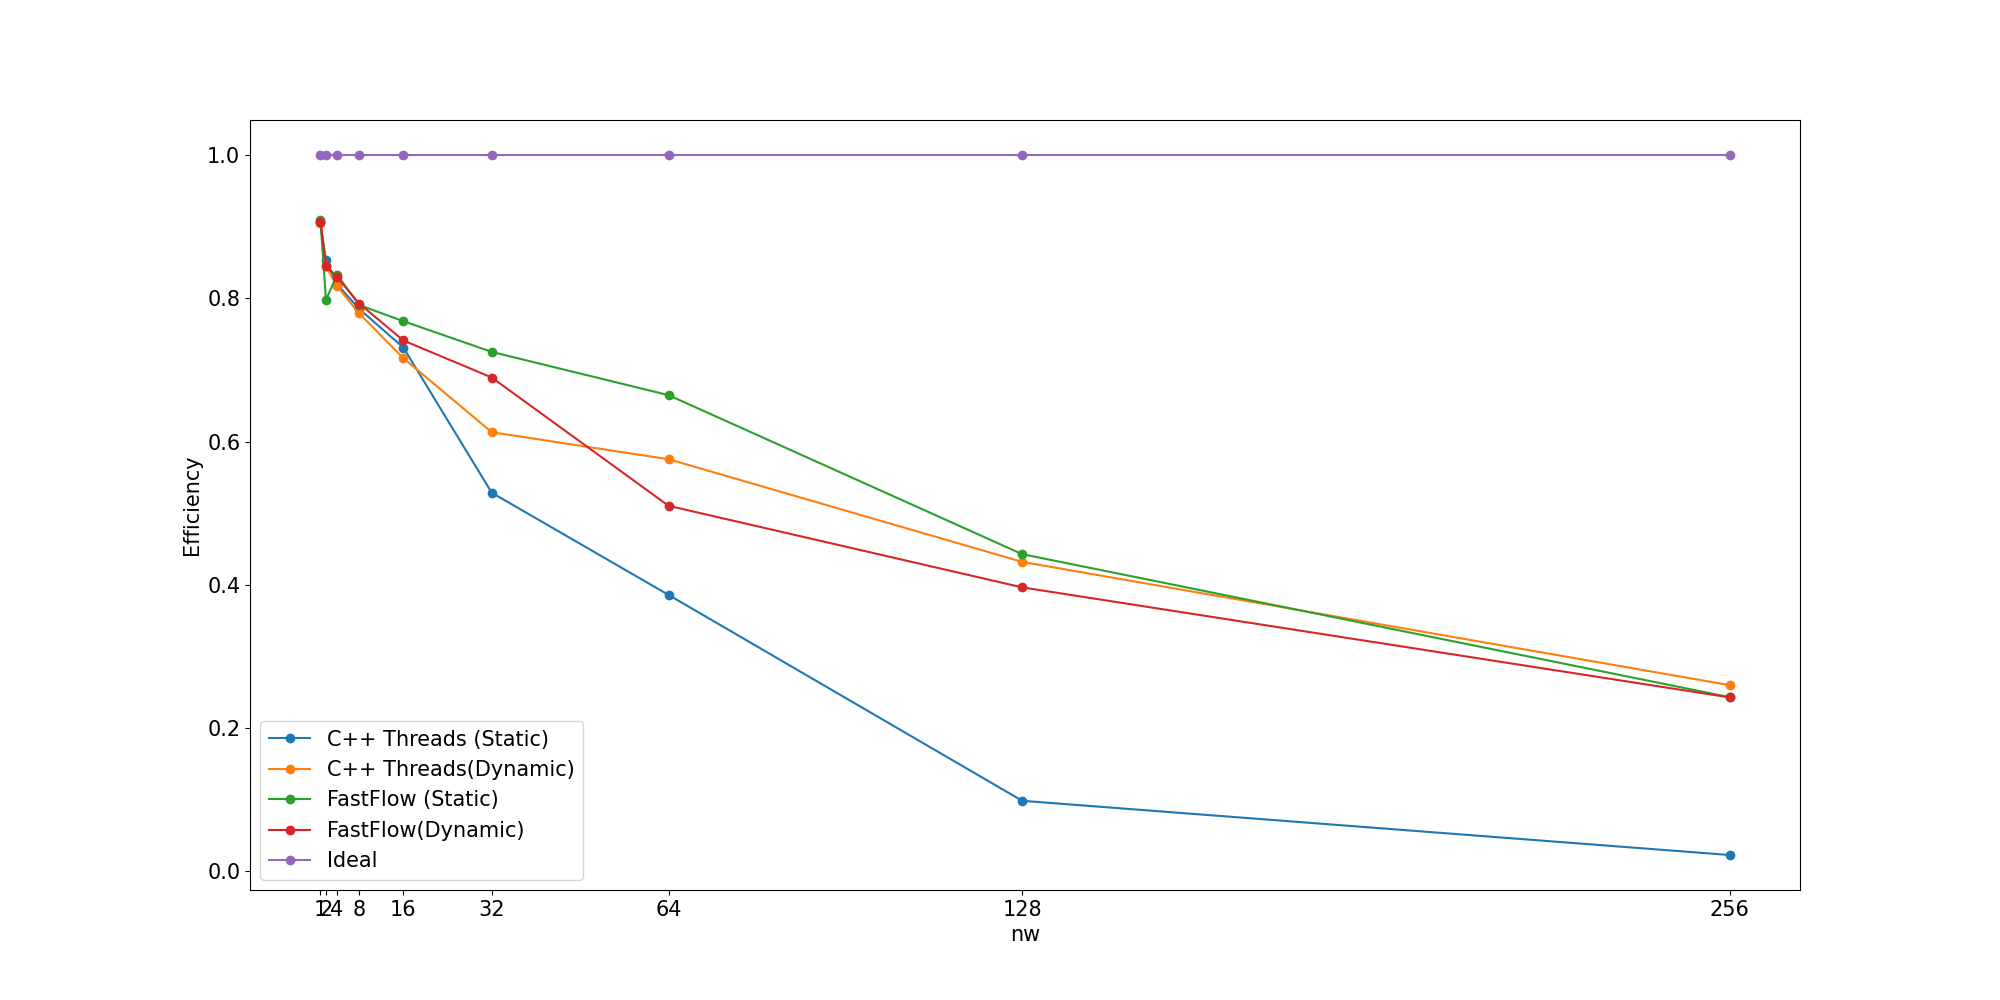
\includegraphics[width=\textwidth]{plots/efficiency.png}
    \caption{Efficiency of the implementations on the Xeon Phi}
    \label{fig:efficiency}
\end{figure}

The efficiency, that decreases very fastly, is plotted in Figure \ref{fig:efficiency}. Here we observe how the FastFlow implementation with static scheduling is also the most efficient one, while all the others suffer a significant overhead. In particular, probabily because of an excessive use of the active-wait queue provided by the library, the FastFlow version with dynamic scheduling is the least efficient (again excluding the C++ Threads outlier).

\begin{figure}
    \centering
    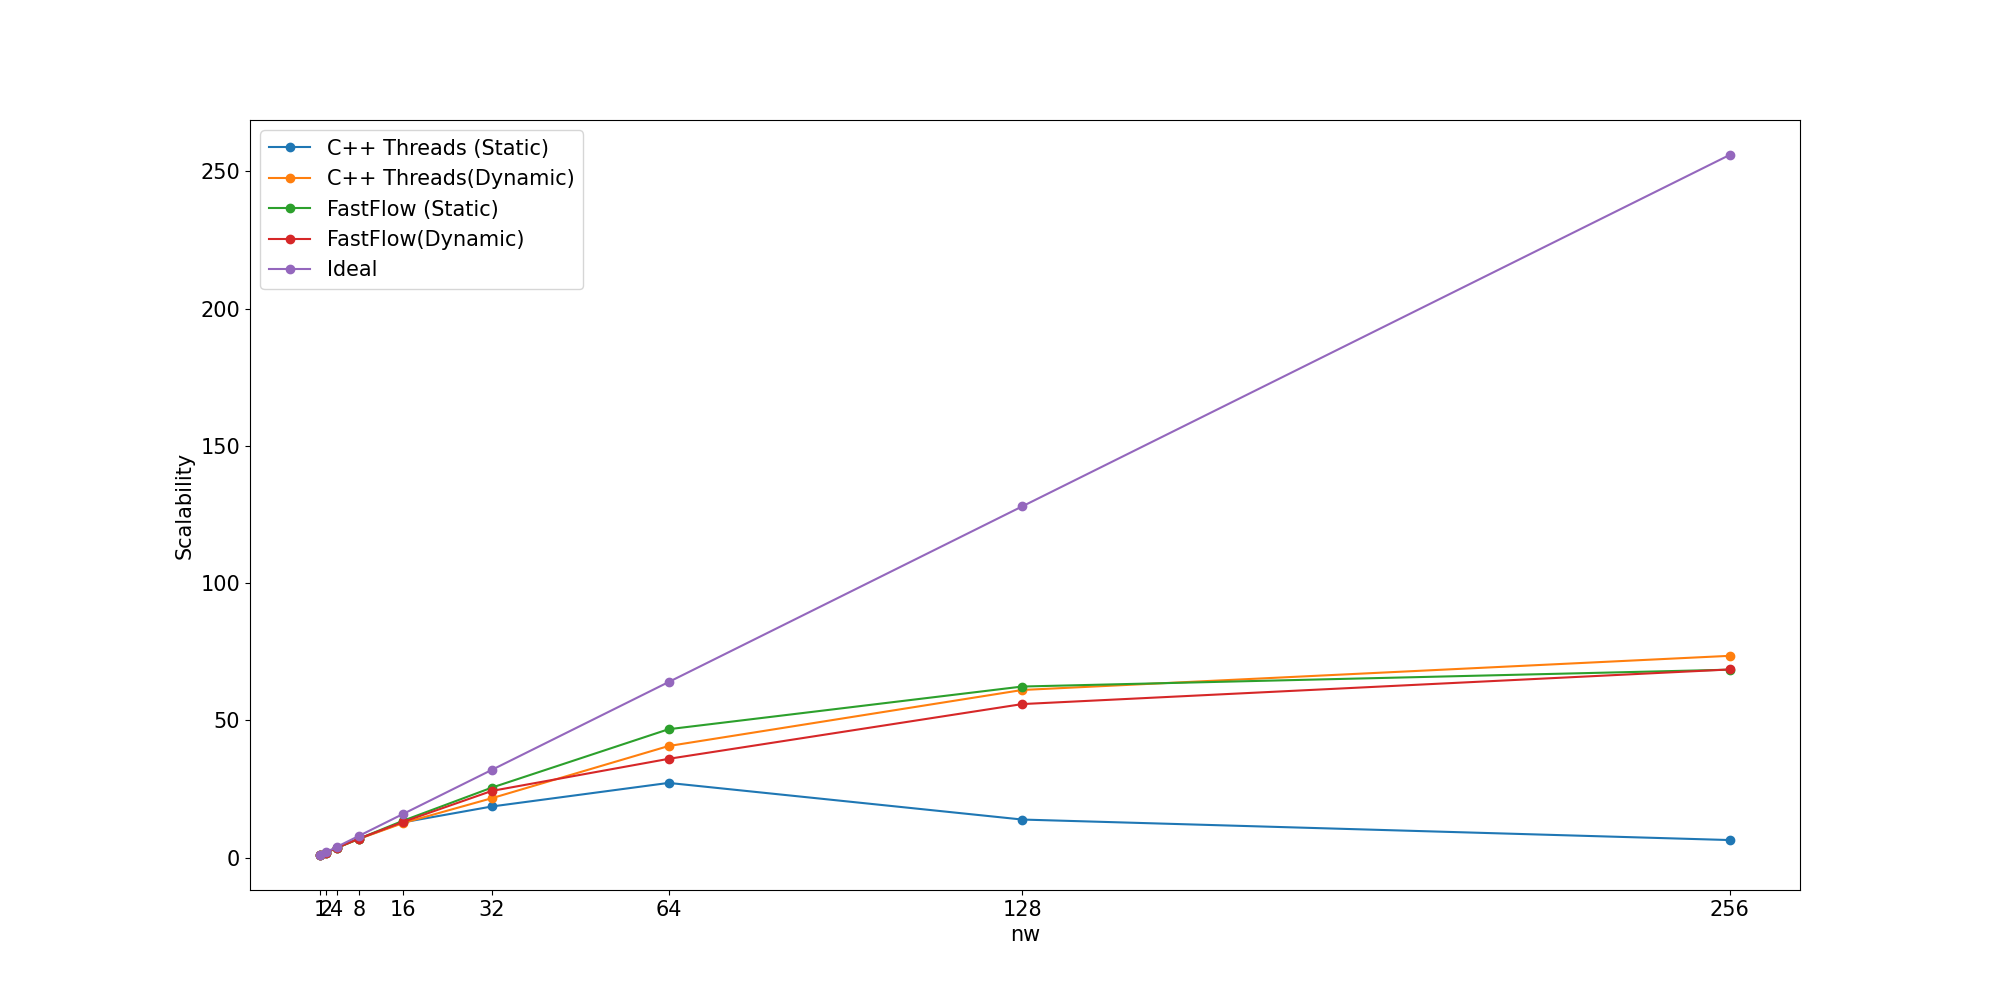
\includegraphics[width=\textwidth]{plots/scalability.png}
    \caption{Scalability on the Xeon Phi}
    \label{fig:scalability}
\end{figure}

Figure \ref{fig:scalability} shows how scalability has the very same behaviour of speedup, with a possible overall winner found in the FastFlow implementation using dynamic scheduling.

\section{Conclusions}

Performing sort of a theoretical analysis, we stated how a parallel implementation cannot scale indefinitely due to the additional operations needed to implement the parallel \texttt{map} and the high dimensionality of the problem. Experiments confirmed that speedup and scalability are bounded by an increasing overhead when the parallelism degree becomes greater, but we didn't reached the point beyond which a parallel version is no more convenient, so we can observe that the parallelization can be effectively exploited even with a large number of processing entities.

For the input data and the available resources taken into account, we found out that the FastFlow implementation using static scheduling is the most convenient, with the dynamic scheduling versions performing slightly worse. The C++ Threads version with static scheduling suffered a very large overhead due to the lack of optimizations needed to better exploit massive multi-core environments, so it's not as convenient as the others.

\end{document}
